\section{Additional Experimental Details}
\label{app:experimental-details}

% NOTE: This appendix is intended to be pasted after the main experimental
% section. It records implementation-level details that are useful for
% reproducibility but would otherwise distract from the main claims in Section 4.
% NOTE: Predictive-isotropy labels were checked against 3method (1).tex:
% lem:predictive_isotropy is the second-moment equivalence and
% thm:predictive_isotropy_opt is the fixed-trace excess-risk minimization result.

\paragraph{Synthetic generator.}
Each synthetic instance is generated from a latent linear--Gaussian model. We
sample a latent vector $s \in \mathbb{R}^{r_\star}$ and observe
\[
    z = C s + \sigma_z \epsilon_z,
    \qquad
    y_k = a_k^\top s + \sigma_y \epsilon_k,
\]
where $C \in \mathbb{R}^{D_x \times r_\star}$ is a randomly sampled
orthonormal context operator, $a_k$ is the $k$th target direction, and the noise
terms are independent isotropic Gaussians. Thus the population predictive
structure is known, but the context coordinates are not aligned with the
canonical basis.

% NOTE: The random orthonormal C avoids the degenerate identity-coordinate case
% while preserving a clean ground-truth predictive subspace for measuring
% recovery.

\paragraph{Target stacks.}
The target operators are constructed in latent space. In the saturation and
bottleneck experiments, we use a complementary target stack whose directions
progressively cover the $r_\star$ latent predictive coordinates. In the
heterogeneity experiment, the construction parameter is chosen so that the
induced population heterogeneity level $\lambda_{\mathrm{het}}$ is sampled
approximately evenly; the plot therefore uses the measured heterogeneity level
directly on the horizontal axis.
In the predictive-isotropy ablation, the target stack is constructed to control
the spectrum directly. For a spectrum decay parameter $\rho\in(0,1]$, we set
\[
    A^\top A
    =
    Q\operatorname{diag}(\lambda_1,\ldots,\lambda_d)Q^\top,
    \qquad
    \lambda_i
    =
    \tau\frac{\rho^{i-1}}{\sum_{j=1}^d\rho^{j-1}},
\]
where $Q$ is a random orthogonal rotation and $\tau$ is fixed across all
conditions. Thus $\operatorname{rank}(A)=d$ and
$\operatorname{tr}(A^\top A)=\tau$ are unchanged, while the measured spectrum
condition
$\kappa_H^2=\lambda_d(H_K)/\lambda_1(H_K)$ ranges from $1$ to approximately
$10^{-8}$. Since the context operator has orthonormal columns and $\sigma_z$ is
fixed, this fixes the nonzero spectrum of $H_K=T_K^\top T_K$ up to the same
scalar context-noise factor across all conditions. The decay parameter $\rho$
is therefore only a generator knob; the figure and interpretation use the
measured operator quantities $\kappa_H^2$ and entropy gap.

% INTERPRETATION: Heterogeneity uses lambda_het as the primary x-axis so the
% appendix plot directly reports the paper's conditioning variable.

\paragraph{Models and estimators.}
We first estimate the unrestricted linear predictor by ordinary least squares
and then compute its rank-$d$ reduced-rank regression approximation by
truncating the singular spectrum. The learned BM-JEPA linear predictor is
therefore the best rank-constrained linear map induced by the finite training
sample. Population curves use the corresponding population cross-covariance
operator under the same target stack and bottleneck dimension.

\paragraph{Metrics.}
All paper-facing MSE panels report average per-target test mean-squared error,
matching the normalization of $\mathcal R_K$ in \eqref{eq:per_target_risk}.
The CSV files also retain fixed-reference-stack diagnostics on a common rich evaluation
target stack as auxiliary representation probes, but these are not the main
risk quantities used in the theory-facing panels. In \cref{fig:heterogeneity},
we show both quantities because they answer different questions: per-target
$\mathcal R_K$ evaluates the changing target stack used for training, whereas
reference-stack MSE evaluates the recovered subspace on a common rich target stack.
As heterogeneity increases, $\mathcal R_K$ can remain nearly constant or rise
slightly because the task becomes less redundant; the reference-stack probe can
decrease at the same time because the recovered subspace becomes more complete.
The standard-error band of $\mathcal R_K$ also shrinks as target coverage spreads
across more latent directions, so the per-target average becomes less dominated
by a single shared direction.
In \cref{fig:predictive-isotropy}, panel (d) uses a related reference-stack probe:
after estimating the top-$d$ right singular subspace of the whitened operator
$\widehat T_K$, we fit a linear predictor from that recovered subspace to a
fixed flat evaluation target stack. This reference-stack excess MSE is not a new
training objective; it is a representation diagnostic showing whether the
recovered predictive subspace captures all latent directions equally well.
For the embedding-versus-predictive isotropy diagnostic, we additionally assign
a synthetic embedding covariance spectrum with eigenvalues proportional to
$\rho_{\mathrm{emb}}^{i-1}$ and fixed trace. This embedding spectrum is varied
independently of the predictive spectrum of $H_K$. It should therefore be read
as a controlled proxy for embedding-level isotropy diagnostics, not as a second
training objective.
Recovered rank is the effective numerical rank of the learned predictor,
computed using a relative singular-value threshold of $0.05$ times the leading
singular value. The heterogeneity metric $\lambda_{\mathrm{het}}$ is the
$r_\star$th nonzero eigenvalue of the target-induced Gram operator. In the
latent coordinates this is the same nonzero spectrum as $A^\top A$; in the
observed context coordinates it is the same nonzero spectrum as
$\Sigma_{ZY}\Sigma_{YZ}$ because $C^\top C=I$. Subspace error is measured by
the largest principal-angle sine between the recovered and true predictive
subspaces.
For the heterogeneity recovery bound, we also compute the empirical
perturbation $\widehat{\epsilon}=\|\widehat{\Sigma}_{YZ}-\Sigma_{YZ}\|_{\rm op}$
and the corresponding Davis--Kahan/Wedin-style denominator
$\sqrt{\lambda_{\mathrm{het}}}-\widehat{\epsilon}$. When this denominator is
nonpositive, the finite-sample bound is vacuous. We keep these quantities in
the CSV as validity diagnostics, but omit them from
\cref{fig:heterogeneity} because the bound is loose for this sweep and is
less informative than the rank and risk panels. The sharper recovery-bound
visualization appears in the post-saturation experiment, where the relative
conditioning condition is non-vacuous over the main finite window.

For the bottleneck experiment, the plotted spectral-tail quantity is the
reduced-rank approximation error predicted by the bottleneck spectral-tail
result:
\[
    \mathcal{E}_{\mathrm{tail}}(d)
    =
    \sum_{j>d} \sigma_j^2,
\]
where $\{\sigma_j\}$ are singular values of the relevant whitened regression
operator. In the figure we report the normalized ratio
$\mathcal{E}_{\mathrm{tail}}(d)/\sum_j\sigma_j^2$ and compare it with the
correspondingly normalized observed excess risk of the rank-$d$ estimator over
the unrestricted OLS estimator.

The rank panel in the bottleneck figure reports the effective rank of the
learned reduced-rank predictor, not the rank of the stacked cross-covariance.
The latter is fixed by the target stack and therefore does not change when the
bottleneck dimension is swept. Since the synthetic target stack has latent
predictive rank $r_\star=24$, a well-estimated rank-$d$ predictor is expected to
use approximately $\min\{d,r_\star\}$ directions. This panel is therefore a
sanity check that the bottleneck cap is the active rank constraint before
$d=r_\star$ and that additional capacity is unused afterward.

% NOTE: The spectral-tail curve is not an additional fitted model. It is
% computed directly from the singular spectrum and compared with observed
% excess risk.

\paragraph{Baselines.}
The main finite-sample baseline is unrestricted OLS, which removes the
embedding bottleneck. Population curves are included as reference predictions
for the same synthetic distribution. The bottleneck experiment additionally
reports a plug-in spectral tail computed from the finite-sample OLS spectrum,
allowing the risk decomposition to be checked using learned empirical
quantities rather than only population quantities.

\paragraph{Configuration summary.}
We list the main Phase-1 configurations used for the reported figures in
\cref{tab:appendix-configs}.

\begin{table}[t]
\centering
\small
\caption{Phase-1 synthetic experiment configurations.}
\label{tab:appendix-configs}
\begin{tabular}{lccccccc}
\hline
Experiment & $n_{\mathrm{train}}$ & $n_{\mathrm{test}}$ & $D_x$ & $r_\star$ & $K$ & $d$ & Noise \\
\hline
$K$ saturation & $1024$ & $8192$ & $160$ & $64$ & sweep & $64$ & $0.12$ \\
Heterogeneity & $32768$ & $8192$ & $64$ & $24$ & $48$ & $24$ & $0.10$ \\
Bottleneck & $128$ & $8192$ & $64$ & $24$ & $48$ & sweep & $0.16$ \\
Post-saturation & $16384$ & $8192$ & $160$ & $64$ & sweep & $64$ & $0.25$ \\
Predictive isotropy & $1024$ & $8192$ & $64$ & $24$ & $24$ & $24$ & $0.25$ \\
Embedding vs. predictive isotropy & $1024$ & $8192$ & $64$ & $24$ & $24$ & $24$ & $0.25$ \\
Gauge factorization & $8192$ & $8192$ & $64$ & $24$ & $24$ & $24$ & $0.25$ \\
\hline
\end{tabular}
\end{table}

\begin{figure}[t]
    \centering
    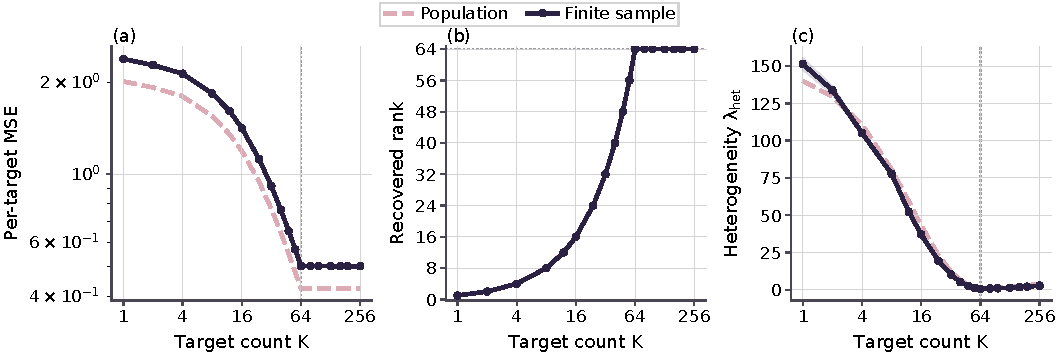
\includegraphics[width=\linewidth]{figures/exp_k_saturation.pdf}
    \caption{$K$-saturation diagnostic. Complementary targets reduce
    per-target MSE and increase recovered rank until predictive rank
    saturates.}
    \label{fig:k-saturation}
\end{figure}

\begin{figure}[t]
    \centering
    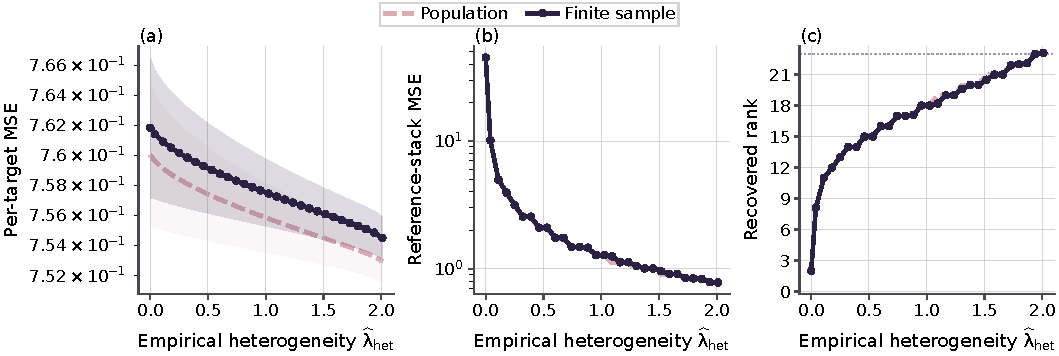
\includegraphics[width=\linewidth]{figures/exp_heterogeneity.pdf}
    \caption{Target-heterogeneity diagnostic. Larger
    $\widehat{\lambda}_{\mathrm{het}}$ improves rank recovery; the
    reference-stack probe measures transfer to a common target stack.}
    \label{fig:heterogeneity}
\end{figure}

\begin{figure}[t]
    \centering
    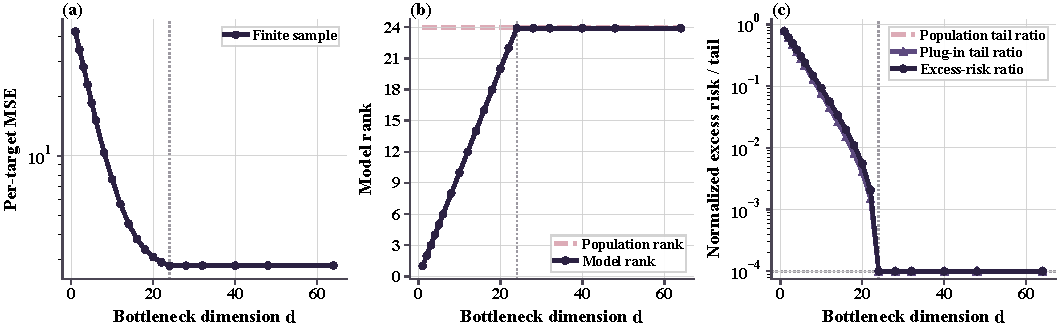
\includegraphics[width=\linewidth]{figures/exp_bottleneck.pdf}
    \caption{Embedding-bottleneck diagnostic. As $d$ increases, model rank
    follows $\min\{d,r_\star\}$ and excess risk tracks the spectral-tail
    ratio.}
    \label{fig:bottleneck}
\end{figure}

\begin{figure}[t]
    \centering
    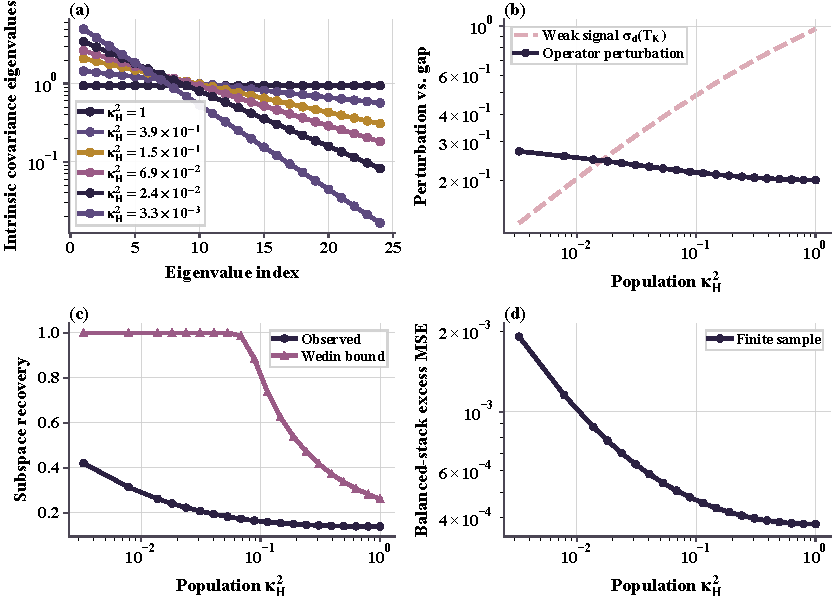
\includegraphics[width=\linewidth]{figures/exp_predictive_isotropy.pdf}
    \caption{Predictive-isotropy diagnostic. At fixed rank and trace, flatter
    spectra of $H_K=T_K^\top T_K$ improve recovery and reduce
    balanced-stack excess MSE.}
    \label{fig:predictive-isotropy}
\end{figure}

\paragraph{Additional theory diagnostics.}
The CSV schema also records the effective rank of the learned RRR coefficient,
the finite-sample target value $\min\{d,\widehat{r}_\star(K)\}$ predicted by
the rank identity, and their difference. This directly checks the rank identity beyond
the displayed rank of the stacked cross-covariance.

The diagnostic in \cref{fig:post-saturation} tests the post-saturation
relative-conditioning mechanism. The target stack is full rank from
$K^\star=d=64$ onward, so
additional targets do not change $r_\star(K)$. The relevant post-saturation
conditioning ratio is
\[
    \kappa_K^2
    =
    \frac{\lambda_d(H_K)}{\lambda_1(H_K)},
    \qquad
    H_K=T_K^\top T_K,\quad
    T_K=\Sigma_{YZ}^{(K)}\Sigma_{ZZ}^{-1/2}.
\]
The initial saturated target stack is deliberately imbalanced. Writing
$A_K^\top A_K$ for the latent target-stack design Gram, we initialize
\[
    A_{K^\star}^\top A_{K^\star}
    =
    Q\operatorname{diag}(c_1,\ldots,c_{64})Q^\top,
\]
where $Q$ is a fixed random orthogonal rotation and
\[
    c_i
    =
    0.02^{(i-1)/63}.
\]
Thus the stack is already rank-$64$, but
$\kappa_{K^\star}^2\approx 0.02$. For $K>K^\star$, each additional target row
is added to the currently weakest eigendirection and contributes $0.1$ units of
target energy. This keeps $r_\star(K)=d$ throughout the plotted window while
increasing $\kappa_K^2$. The finite-sample subspace error and per-target excess
MSE decrease over the same window, supporting the repaired post-saturation
claim that extra targets help only when they improve relative conditioning of
the already-accessible predictive subspace.
In \cref{fig:post-saturation}, we keep the core post-saturation diagnostics in
the first row: the weakest and top eigenvalues of $H_K=T_K^\top T_K$ in a
shared panel, the relative conditioning ratio $\kappa_K^2$, and the effective
dimension of $T_K$. The
second row reports the risk-stability bound, excess risk, and finite-sample
risk. The
effective-dimension panel checks that
$\operatorname{effdim}(T_K)$ remains bounded over the finite
window in the finite-window post-saturation relative-geometry condition. To instantiate the
risk-stability constant, we compute the empirical ratio
\[
    \widehat L_K
    =
    \frac{[\widehat{\mathcal R}_K-\mathcal R_K^\star]_+}
    {\|\sin\Theta(V_K,\widehat V_K)\|_{\mathrm{op}}},
\]
using per-target excess MSE in the numerator, and set
$\widehat L=\max_{K,\mathrm{seed}}\widehat L_K$. Panel (d) then plots the
excess-risk left-hand side against the empirical bound curve
$\widehat L\|\sin\Theta(V_K,\widehat V_K)\|_{\mathrm{op}}$, matching the form of
the normalized risk-stability condition. Each seed is one
deterministic draw of the synthetic data and target stack, and the same
$\widehat L$ is used across the full plotted window. In the current run this
gives $\widehat L=7.07\times10^{-3}$.

For the concentration constant in \eqref{eq:post_saturation_epsilon}, we set
$\delta=0.1$ and compute
\[
    a_K
    =
    \sqrt{\frac{\operatorname{effdim}(T_K)+\log(1/\delta)}{n}},
    \qquad
    \widehat{\eta}_K
    =
    \frac{\|\widehat T_K-T_K\|_{\mathrm{op}}}{\|T_K\|_{\mathrm{op}}}.
\]
We then set $\widehat C_{0.9}$ to the $90$th percentile, over all plotted
$(K,\mathrm{seed})$ pairs, of $\widehat{\eta}_K/a_K$. This gives
$\widehat C_{0.9}=1.79$ and covers $90/100$ normalized perturbation samples by
construction. Panel (e) uses the calibrated bound
\[
    \frac{2\widehat L\widehat C_{0.9}a_K}{\kappa_K}
\]
from \eqref{eq:post_saturation_excess_risk_bound}. Panel (f) adds this term to
the population OLS risk estimate, matching the risk-decomposition bound in
\cref{prop:post_saturation_risk}. In this post-saturation setting
$d=r_\star(K)$, so the spectral-tail term is zero up to numerical precision.

% NOTE: Post-saturation labels were checked against 3method (1).tex.
To check that the simplified rate is not vacuous in the plotted regime, we
evaluate the empirical analogue of the half-gap condition in
\eqref{eq:post_saturation_half_gap}. Define the normalized perturbation
\[
    \widehat{\eta}_K
    :=
    \frac{\|\widehat T_K-T_K\|_{\mathrm{op}}}
    {\|T_K\|_{\mathrm{op}}}.
\]
The condition $\widehat{\eta}_K\le \kappa_K/2$ holds seed-wise for all
deterministic runs in the plotted range. The weakest endpoint, $K=64$, is
deliberately closest to the small-conditioning boundary and remains just inside
the half-gap window for the current sample size.
Representative values are:
\[
\begin{array}{c|cccc}
K & \widehat{\eta}_{K,\mathrm{mean}} & \widehat{\eta}_{K,\max}
  & \kappa_K/2 & \mathrm{valid\ seeds} \\
\hline
64 & 0.0613 & 0.0656 & 0.0707 & 10/10 \\
96 & 0.0626 & 0.0688 & 0.1751 & 10/10 \\
512 & 0.0929 & 0.0947 & 0.4748 & 10/10
\end{array}
\]

As an appendix-only diagnostic, we also substitute the same
$\widehat C_{0.9}$ into the intermediate Wedin-style recovery bound from the
proof of \cref{cor:post_saturation_relative_rate}. This yields the dashed
subspace-recovery curve in
\cref{fig:post-saturation-recovery-bound}. The induced curve is conservative:
it covers all observed $\|\sin\Theta_T\|_{\mathrm{op}}$ values in the plotted
window, because the deterministic perturbation step is looser than the empirical
perturbation quantile.

\begin{figure}[t]
    \centering
    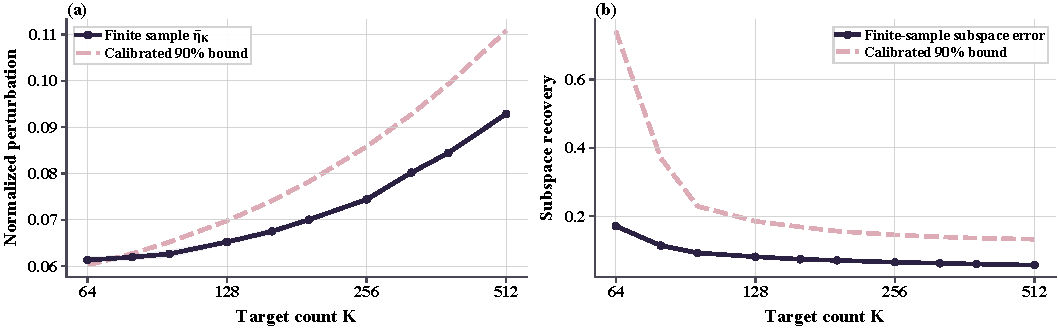
\includegraphics[width=\linewidth]{figures/exp_post_saturation_recovery_bound.pdf}
    \caption{Post-saturation recovery-bound calibration. The calibrated
    perturbation bound is conservative but covers the observed subspace error.}
    \label{fig:post-saturation-recovery-bound}
\end{figure}

\paragraph{Predictive-isotropy construction.}
The fixed-trace predictive-isotropy experiment is designed to test the
second-moment prediction in \cref{lem:predictive_isotropy} and the
fixed-trace bound minimization in
\cref{thm:predictive_isotropy_opt}, without changing rank or total
signal energy.
All conditions use $D_x=64$, $r_\star=d=K=24$,
$\sigma_z=\sigma_y=0.25$, and
$\operatorname{tr}(H_K)=22.59$ after the common whitening/context-noise scaling.
The generator uses 20 decay values between $\rho=1.00$ and $\rho=0.78$,
concentrated near the transition where the weakest retained signal becomes
comparable to the empirical perturbation scale.
They induce a dense sweep of population conditioning values
$\kappa_H^2\in[3.30{\times}10^{-3},1]$. Representative points are:
\[
\begin{array}{c|ccc}
\rho & \kappa_H^2 & \mathrm{entropy\ gap}
& \|\sin\Theta_T\|_{\mathrm{op}} \\
\hline
1.00 & 1.0000 & 0.000 & 0.139 \\
0.94 & 2.41{\times}10^{-1} & -0.090 & 0.146 \\
0.90 & 8.86{\times}10^{-2} & -0.253 & 0.165 \\
0.86 & 3.12{\times}10^{-2} & -0.495 & 0.207 \\
0.84 & 1.81{\times}10^{-2} & -0.644 & 0.241 \\
0.78 & 3.30{\times}10^{-3} & -1.191 & 0.420
\end{array}
\]
The trace column is omitted because it is constant by construction. Since
$\widetilde Z=\Sigma_{ZZ}^{-1/2}Z$ is Gaussian in this generator, the intrinsic
covariance of $P_K=T_K\widetilde Z$ on its rank-$d$ range has eigenvalues
$\lambda_i(H_K)$. Thus panel (a) of \cref{fig:predictive-isotropy} is directly
the covariance spectrum appearing in \cref{lem:predictive_isotropy}. Panel (b)
plots the two quantities that determine the perturbative denominator:
$\sigma_d(T_K)$ and $\|\widehat T_K-T_K\|_{\mathrm{op}}$. Panel (c) compares
the observed subspace recovery error with the Wedin bound
$\|\widehat T_K-T_K\|_{\mathrm{op}}/
(\sigma_d(T_K)-\|\widehat T_K-T_K\|_{\mathrm{op}})$, clipped at one when the
denominator is nonpositive. The small-$\kappa_H^2$ settings intentionally enter
this vacuous-bound regime; they show the transition from perturbative recovery
to the boundary where weak directions begin to become difficult to recover. In
the current ten-seed run, 16 of the 20 spectrum settings have a positive
perturbative denominator for every seed, and 10 of 20 satisfy the half-gap
diagnostic for every seed.

\paragraph{Embedding versus predictive isotropy.}
The embedding-versus-predictive diagnostic varies two spectra independently:
the synthetic embedding covariance spectrum and the predictive spectrum of
$H_K=T_K^\top T_K$. The embedding decay values are
$\rho_{\mathrm{emb}}\in\{1.00,0.65,0.45\}$, and the predictive decay values are
$\rho_{\mathrm{pred}}\in\{1.00,0.85,0.65,0.45\}$. Both spectra are normalized to
the same trace within their own space. This creates cases with nearly isotropic
embedding covariance but badly conditioned predictive operator, and cases with
anisotropic embedding covariance but well-conditioned predictive operator.

\cref{fig:embedding-vs-predictive-isotropy} reports the result. Averaging over
predictive spectra, the reference-stack excess MSE is unchanged across the three
embedding decay values, while changing the predictive spectrum changes the
subspace-recovery and reference-stack diagnostics. This does not claim that
embedding isotropy is useless in nonlinear JEPA training; it shows that
embedding isotropy is not the operator-level quantity appearing in the
finite-sample recovery bound.
The fair interpretation is therefore complementary: embedding isotropy controls
the marginal representation law, while predictive isotropy controls the
target-conditioned end-to-end signal. In the notation of the theory draft,
encoder-side regularization acts on the pushforward $\mathcal L(AZ)$, whereas
predictive isotropy acts on the prediction-aware pushforward
$\mathcal L(P_K)$ with $P_K=T_K\widetilde Z$. These coincide only under special
coverage conditions; in general, a representation can be marginally isotropic
while the target-predictive operator remains highly anisotropic.

\begin{figure}[t]
    \centering
    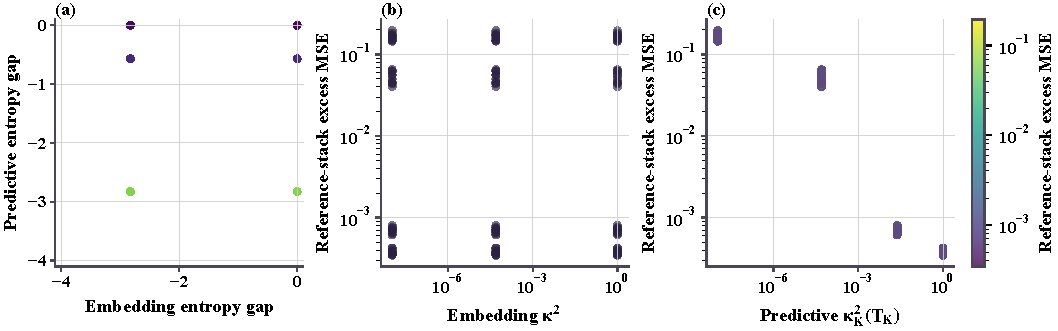
\includegraphics[width=\linewidth]{figures/exp_embedding_vs_predictive_isotropy.pdf}
    \caption{Embedding versus predictive isotropy. Predictive conditioning
    tracks the reference-stack probe more directly than marginal embedding
    conditioning.}
    \label{fig:embedding-vs-predictive-isotropy}
\end{figure}

\paragraph{Gauge-factorization diagnostic.}
The gauge diagnostic directly targets \cref{subsubsec:gauge_factorization}.
For each seed, we construct the population whitened predictor
$T_K=U_KS_KV_K^\top$ and compare identity, random orthogonal, anisotropic
diagonal, and nonlinear Gaussianizing gauges under both Gaussian and
standardized Laplace SVD-coordinate distributions. For an invertible linear
gauge $G$, the synthetic encoder and predictor are
\[
    \Lambda_G(Z)=G V_K^\top\Sigma_{ZZ}^{-1/2}Z,
    \qquad
    F_G(\cdot)=U_KS_KG^{-1}(\cdot).
\]
Panel (a) of \cref{fig:gauge-factorization} verifies
\cref{lem:gauge_invariance}: all gauges reproduce the same end-to-end
prediction up to numerical precision. Panel (b) checks the covariance part of
\cref{thm:subsumes_cov_isotropy}: identity and orthogonal gauges remain
covariance-isotropic up to finite-sample error for both context laws, while the
diagonal gauge is deliberately anisotropic. Panel (c) reports a
Cramer--Wold-style projected standard-normal discrepancy. For Gaussian context,
the identity/SVD-aligned gauge already realizes the linear-Gaussian special
case in \cref{cor:linear_gauss}. For Laplace context, identity remains
covariance-isotropic but not Gaussian; the nonlinear Gaussianizing gauge maps
the intrinsic coordinates to standard-normal marginals and sharply reduces the
projected discrepancy, illustrating the role of the nonlinear gauge in
\cref{thm:subsumes_gaussian_isotropy}.

\begin{figure}[t]
    \centering
    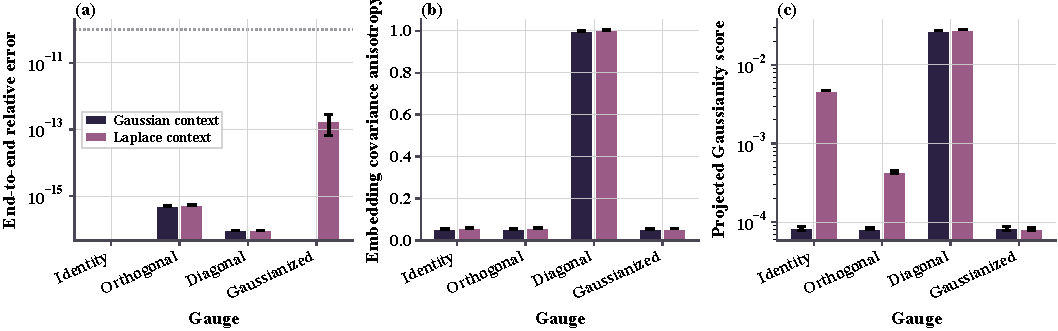
\includegraphics[width=\linewidth]{figures/exp_gauge_factorization.pdf}
    \caption{Gauge-factorization diagnostic. Gauge changes preserve prediction
    while changing encoder covariance and Gaussianity diagnostics.}
    \label{fig:gauge-factorization}
\end{figure}

\paragraph{Regularization implication.}
The revised theory proposes a prediction-aware analogue of embedding-side
Gaussian regularization. Standard embedding regularizers act on the marginal
pushforward $\mathcal L(AZ)$, whereas the theory-facing object here is the
intrinsic end-to-end predictive pushforward from
\cref{lem:predictive_isotropy}. For a minibatch, project the learned predicted
outputs onto the learned rank-$d$ predictive range and collect the intrinsic
coordinates into rows $\widehat p_n^{\mathrm{int}}$ of
\[
    \widehat P^{\mathrm{int}} \in \mathbb{R}^{N\times d}.
\]
The proposed regularizer samples random directions
$\mathcal A\subset\mathbb S^{d-1}$ and averages a univariate Gaussianity test,
such as the Epps--Pulley statistic, over the projected samples:
\[
    \mathcal R_{\mathrm{PI}}(\widehat P^{\mathrm{int}};\mathcal A)
    =
    \frac{1}{|\mathcal A|}
    \sum_{u\in\mathcal A}
    \mathcal T\!\left(\{u^\top \widehat p_n^{\mathrm{int}}\}_{n=1}^N\right).
\]
This is a Cramer--Wold-style, prediction-aware counterpart to SIGReg: it acts
on intrinsic predictor outputs rather than encoder embeddings. Matching
projected standard normals is stronger than the second-moment condition
$H_K=\alpha I$, but it implies the isotropic predictive covariance targeted by
\cref{lem:predictive_isotropy}. A practical nonlinear objective could therefore
take the schematic form
\[
    \mathcal L
    =
    \mathcal L_{\mathrm{pred}}
    +
    \lambda_{\mathrm{emb}}\mathcal L_{\mathrm{emb\text{-}iso}}
    +
    \lambda_{\mathrm{pred}}\mathcal R_{\mathrm{PI}}.
\]
The first regularizer is task-agnostic and prevents marginal representation
collapse; the second is task-conditioned and targets the predictive spectrum
appearing in the finite-sample recovery and excess-risk bounds. The gauge
results in the theory explain why a sufficiently strong prediction-aware
regularizer can subsume encoder-side isotropy at the population level; in
practice, the two terms may still be combined for optimization and collapse
prevention.

The experiments in
\cref{fig:predictive-isotropy,fig:embedding-vs-predictive-isotropy} validate
the second-moment spectral mechanism behind this proposal. The next diagnostic
tests the corresponding regularizer in a learned nonlinear predictor.

\paragraph{Digits regularizer experiment.}
We add a low-label real-data training diagnostic on the
\texttt{sklearn} handwritten-digits dataset. The context is the left half of
the $8\times 8$ digit image and the target is the right half. A nonlinear
encoder maps the context to a $16$-dimensional embedding; a predictor maps this
embedding to a $16$-dimensional intrinsic prediction representation; a final
linear head predicts the target pixels. We identify this predictor
representation with the finite-network analogue of
$\widehat P_K^{\mathrm{int}}$ in
\eqref{eq:predictive_isotropy_regularizer}; the pixel head is only the readout
used to evaluate target prediction. To make generalization rather than
in-sample reconstruction the limiting factor, we train a high-capacity model on
only an $8\%$ stratified training split and evaluate on the remaining examples.
We compare four objectives: no regularizer, an encoder-only Gaussianity
penalty, a prediction-only Gaussianity penalty, and a prediction-plus-encoder
auxiliary condition. The projected-Gaussianity term combines the
Cramer--Wold/Epps--Pulley statistic with a covariance-to-identity penalty, and
is applied either to the encoder embedding or to the prediction representation.
The prediction-plus-encoder condition is included as a control: the theory
predicts that the prediction-side condition is the risk-relevant one, so adding
an encoder-side auxiliary penalty should not be necessary for the main risk
effect.

\Cref{fig:regularizer-digits} and \cref{tab:regularizer-digits-cost} show the
result over ten deterministic seeds.
Here MSE is the primary criterion. It is the mean squared error over right-half
target pixels after normalizing digit intensities to $[0,1]$; it is not a
percentage. The corresponding RMSE can be read as a fraction of the full
gray-scale range.
The Gaussianity score is only a diagnostic: it is a distance from projected
standard-normal laws, so smaller values mean the regularizer has moved the
intended distribution, but this score is not a substitute for test risk.
Effective rank is likewise a conditioning diagnostic, not a standalone
objective. In this harder setting, prediction-side regularization reduces test
MSE from $9.23{\times}10^{-2}$ to
$6.00{\times}10^{-2}$ and the train--test gap from $8.54{\times}10^{-2}$ to
$2.00{\times}10^{-2}$. The same runs reduce predictive Gaussianity distance
from $1.14{\times}10^{-1}$ to $4.33{\times}10^{-2}$ and raise predictive
effective rank from $4.13$ to $6.41$. Encoder-side regularization also improves
test MSE, but less strongly, and it does not improve the prediction-side
Gaussianity distance. The prediction-only and prediction-plus-encoder
conditions have nearly identical test MSE, which is the expected control outcome
under the subsumption result. The timing panel makes the cost tradeoff explicit:
prediction-side regularization takes $12.23$ seconds per seed on average,
compared with $9.03$ seconds for no regularizer and $15.80$ seconds for the
combined objective. Thus the prediction-side term gives essentially the same
test risk as the combined condition at lower cost. This experiment is not meant
to replace large-scale JEPA validation, but
it does test the proposed regularizer inside an actual learned nonlinear
predictor rather than a closed-form synthetic operator.
\Cref{fig:regularizer-digits-samples} gives a qualitative view of the same
task: the left half of each test digit is observed, and each method predicts the
right half.

\begin{figure}[t]
    \centering
    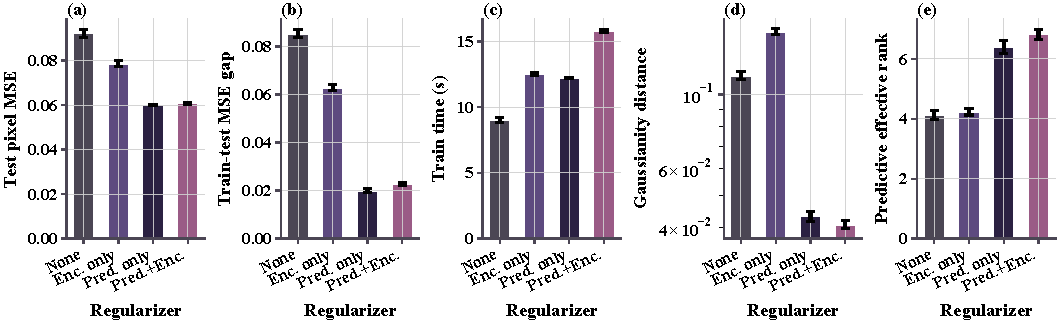
\includegraphics[width=\linewidth]{figures/exp_regularizer_digits.pdf}
    \caption{Digit regularizer diagnostics. Prediction-side regularization
    gives the best pixel-MSE/generalization tradeoff and improves
    prediction-side conditioning diagnostics.}
    \label{fig:regularizer-digits}
\end{figure}

% NOTE: In a nonlinear JEPA implementation, \widehat P can be taken as the
% stacked predictor outputs before the target loss. A stop-gradient choice may
% be needed if one wants this term to regularize the predictor/context pathway
% without directly reshaping the teacher targets.

% NOTE: The rotation prevents a coordinate-axis artifact; the eigenvalues of
% the latent design Gram are unchanged, but the observed context coordinates are random.
% INTERPRETATION: This is a finite-window diagnostic. Since kappa_K^2 <= 1, the
% trend cannot continue indefinitely and should not be presented as an
% asymptotic-in-K law. The stability-ratio panel is an empirical diagnostic, not
% an independent proof of a global Lipschitz constant L.

\paragraph{Reproducibility.}
All Phase-1 experiments are run with ten deterministic seeds. The full
synthetic suite can be reproduced with
\[
    \texttt{python -m experiments.run\_all}
\]
followed by
\[
    \texttt{python -m plots.plot\_main}.
\]
The qualitative digit reconstruction figure is generated separately with
\[
    \texttt{python -m plots.plot\_regularizer\_digits\_samples}.
\]
The scripts write per-experiment CSV files, the combined result table, and the
main and appendix PDF figures. Unit tests cover deterministic generation,
OLS/RRR behavior, rank constraints, subspace metrics, CSV schema, and
figure-reference existence.

\paragraph{Visualization choices.}
Finite-sample estimates are plotted as solid curves with standard-error bands.
Population predictions are plotted as dashed gray curves.
For the bottleneck spectral-tail-ratio panel, values below $10^{-4}$ are
visually floored in the log-scale display to keep the super-threshold regime
legible; this affects only the display, not the CSV values or computations.

% INTERPRETATION: The visual floor prevents near-zero numerical tails from
% dominating the axis while still showing that the post-bottleneck tail
% vanishes.
